\iffalse
\documentclass[10pt,a4paper]{report}
\usepackage[latin1]{inputenc}
\usepackage{amsmath}
\usepackage{amsfonts}
\usepackage{amssymb}
\usepackage{graphicx}
\usepackage{hyperref}
\usepackage{multicol}
\usepackage[margin=0.5in]{geometry}
\usepackage{tikz}
\usepackage[document]{ragged2e}
\usepackage{romannum}
\usetikzlibrary{arrows,shapes.gates.logic.US,shapes.gates.logic.IEC,calc}
\usepackage{titlesec}
\titlespacing{\subsection}{1pt}{\parskip}{3pt}
\titlespacing{\subsubsection}{0pt}{\parskip}{-\parskip}
\titlespacing{\paragraph}{0pt}{\parskip}{\parskip}
\newcommand{\myvec}[1]{\ensuremath{\begin{pmatrix}#1\end{pmatrix}}}
\let\vec\mathbf

\newcommand{\mydet}[1]{\ensuremath{\begin{vmatrix}#1\end{vmatrix}}}
\providecommand{\brak}[1]{\ensuremath{\left(#1\right)}}
\providecommand{\lbrak}[1]{\ensuremath{\left(#1\right.}}
\providecommand{\rbrak}[1]{\ensuremath{\left.#1\right)}}
\providecommand{\sbrak}[1]{\ensuremath{{}\left[#1\right]}}

\begin{document}

\begin{multicols}{2}
\raggedright {\includegraphics[scale=0.06]{iith_logo.png}} \vspace{3mm}\\ \raggedleft Hari Venkateswarlu Annam\vspace{2mm}\\ 
\raggedleft  FWC22058\vspace{2mm}\\ 
\raggedleft hariannam99@gmail.com \vspace{2mm}\\ 
\raggedleft Oct 2022 \vspace{5mm}\\
\end{multicols}

\centering \Large \textbf{MATRIX : CONIC ASSIGNMENT} \normalsize \vspace{10mm}

\begin{multicols}{2}

\section{Problem:}  
\fi
Find the area between the curves $y=x$ and $y=x^2$.
\\
\solution
	\begin{figure}[!h]
		\centering
 \includegraphics[width=\columnwidth]{chapters/12/8/3/2/figs/figure.png}
		\caption{}
		\label{fig:12/8/3/2}
  	\end{figure}
\iffalse
\section{Solution: }
\raggedright \textbf{Input Parameters :}\\ \vspace{2mm}
\centering Curve Equation : $y=x^2$. \\ \vspace{1mm}
Line Equation : $y=x$.\\
\vspace{3mm}

\raggedright \textbf{To Find :}\\ \vspace{2mm}
\begin{enumerate}
\item Comparing the given curve equation with the standard equation of the conics and finding it's parameters.
\item Finding the required parameters for the line equation.
\item Finding the Point of Intersection of the to the curve.
\item Finding the area between the curve.
\end{enumerate}

\raggedright \textbf{Step - 1 :}\\ \vspace{2mm}
Curve Equation : $y=x^2$. \\ \vspace{1mm}
The standard equation of the conics is given as :
\begin{align}
\vec{x}^{\top}\vec{V}\vec{x}+2\vec{u}^{\top}\vec{x}+f=0
\end{align}
\fi
The given curve  can be expressed as a conic with parameters
\begin{align}
	\vec{V} &= \myvec{1 & 0\\0 & 0}, \vec{u} = \myvec{0 \\-\frac{1}{2}}, f = 0
	\end{align}
\iffalse
\raggedright \textbf{Step - 2 :}\\ \vspace{2mm}
Line Equation : $y=x$. \\ \vspace{1mm}
From the above line equation below vectors are taken
\fi
The given line parameters are
\begin{align}
\vec{h} = \myvec{0 \\0}, \vec{m}=\myvec{1\\1}
\end{align}
\iffalse

\raggedright \textbf{Step - 3 :}\\ \vspace{2mm}
The points of intersection of the line, \\ 
\begin{align}
L: \quad \vec{x} = \vec{q} + \mu \vec{m} \quad \mu \in \mathbb{R}
\end{align}
with the conic section, \\ 
\begin{align}
	\vec{x}^{\top}\vec{V}\vec{x} + 2\vec{u}^{\top} \vec{x} + f = 0
\end{align}
are given by \\
\begin{align}
\vec{x}_i = \vec{q} + \mu_i \vec{m}
\end{align}
where, \\
{\tiny
\begin{multline}
\mu_i = \frac{1}
{
\vec{m}^T\vec{V}\vec{m}
}
\lbrak{-\vec{m}^T\brak{\vec{V}\vec{q}+\vec{u}}}
\\
\pm
\rbrak{\sqrt{
\sbrak{
\vec{m}^T\brak{\vec{V}\vec{q}+\vec{u}}
}^2
-
\brak
{
\vec{q}^T\vec{V}\vec{q} + 2\vec{u}^T\vec{q} +f
}
\brak{\vec{m}^T\vec{V}\vec{m}}
}
}
\end{multline}
}
\raggedright On substituting $\vec{V},\vec{q} ,\vec{m}$ in the above equation,
we get the values of $\mu$. By substituting the values of $\mu$ in eq(6), \\we get the points of intersection of line with the given curve. \\
\centering $i.e., \vec{x_1},\vec{x_2}$\\ 
\fi
Substituting the given parameters in 
\eqref{eq:tangent_roots},
\begin{align}
\vec{x_1}=\myvec{0\\0}, \vec{x_2}=\myvec{1\\1}.
\end{align}
From Fig. 
		\ref{fig:12/8/3/2},
the area bounded by the curve $y=x^2$ and line $y=x$ is given by
\begin{align}
	\int_{0}^{1} \brak{x 
	-\frac{x^2}{2}} \,dx = \frac{1}{6}
\end{align}
\iffalse

\centering By solving we get the required area\\
$\therefore A = \frac{1}{6}$ 



\section{Termux Commands :}
\centering bash rncom.sh ..... Using Shell commands.


\section{Plot :} 
\begin{center}
  \includegraphics[scale=0.55]{figure.png}
  	\end{center}

 
\end{multicols}
\end{document}
\fi
